%\documentstyle[epsf,twocolumn]{jarticle}       %LaTeX2e仕様
%\documentclass[twocolumn]{jarticle}     %pLaTeX2e仕様(platex.exeの場合)
\documentclass[onecolumn]{ujarticle}     %pLaTeX2e仕様(uplatex.exeの場合)
%%%%%%%%%%%%%%%%%%%%%%%%%%%%%%%%%%%%%%%%%%%%%%%%%%%%%%%%%%%%%%
%%
%%  基本バージョン
%%
%%%%%%%%%%%%%%%%%%%%%%%%%%%%%%%%%%%%%%%%%%%%%%%%%%%%%%%%%%%%%%%%
\setlength{\topmargin}{-45pt}
%\setlength{\oddsidemargin}{0cm} 
\setlength{\oddsidemargin}{-7.5mm}
%\setlength{\evensidemargin}{0cm} 
\setlength{\textheight}{24.1cm}
%setlength{\textheight}{25cm} 
\setlength{\textwidth}{17.4cm}
%\setlength{\textwidth}{172mm} 
\setlength{\columnsep}{11mm}

%\kanjiskip=.07zw plus.5pt minus.5pt


% 【節が変わるごとに (1.1)(1.2) … (2.1)(2.2) と数式番号をつけるとき】
%\makeatletter
%\renewcommand{\theequation}{%
%\thesection.\arabic{equation}} %\@addtoreset{equation}{section}
%\makeatother

%\renewcommand{\arraystretch}{0.95} 行間の設定

%%%%%%%%%%%%%%%%%%%%%%%%%%%%%%%%%%%%%%%%%%%%%%%%%%%%%%%%
%\usepackage{graphicx}   %pLaTeX2e仕様(\documentstyle ->\documentclass)
\usepackage[dvipdfmx]{graphicx}
\usepackage{subcaption}
\usepackage{multirow}
%%%%%%%%%%%%%%%%%%%%%%%%%%%%%%%%%%%%%%%%%%%%%%%%%%%%%%%%
\begin{document}
	
	%bibtex用の設定
	%\bibliographystyle{ujarticle} 
	
	\noindent
	
	\hspace{1em}
	2019 年 4 月 26 日
	ゼミ資料
	\hfill
	M1 寺内 光
	
	\vspace{2mm}
	
	\hrule
	
	\begin{center}
		{\Large \bf 進捗報告}
	\end{center}
	
	
	\hrule
	\vspace{3mm}
	
	% ‚ここから 文章 Start!
	\section{今週確認したこと}
	モデル構造を変更し,中間層の出力サイズの変更を行った.元画像サイズ(196, 136)だったのを(208, 128)に変更.この変更によって MAX プーリングが 2 回→ 4 回かけられるようになった. 
	
	実験として中間層の shape (13, 8) に対して filter数 を変化させたときのタッチ識別の accuracy の変化を確認.表 \ref{tab:classify_n_filter}, 図 \ref{fig:classify_n_filter} にその結果を示す.また,識別器に用いたのはすべて Random Forest である.
	\begin{table}[h]
		\centering
		\caption{filter 数を変化させたときのaccuracyの変化}
		\begin{tabular}{|c|c|c|c|c|c|c|} \hline
			-&1&2&4&8&16&32\\ \hline\hline
			test&0.556&0.624&0.725&0.729&0.786&0.745\\ \hline
			train&0.417&0.542&0.563&0.604&0.583&0.667\\ \hline
		\end{tabular}
		\label{tab:classify_n_filter}
	\end{table}

	\begin{figure}[h]
		\begin{center}
			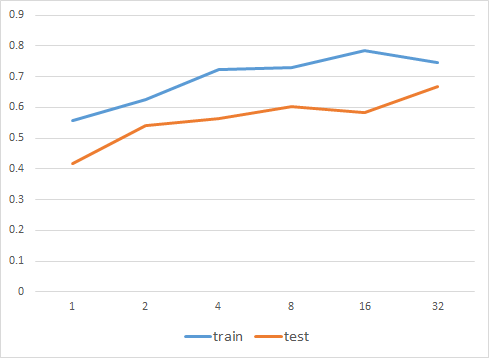
\includegraphics[width=0.8\columnwidth]{n_filter.png}
			\caption{filter 数を変化させたときのaccuracyの変化}
			\label{fig:classify_n_filter}
		\end{center}
	\end{figure}

	\section{計算機サーバのセットアップ}
	昨日,実 30 時間労働の末,届いた計算機サーバ (kanonserv) のセットアップが完了した.
	また知見としてセットアップ手順をまとめて github にあげる予定.

	\section{来週の予定}
	\begin{itemize}
		\item PFN インターンのコーディング課題(Web アノテーションツール).
		\item 新しいモデルの構想
		\item zope のブログ用ページの試作 (markdown に対応できるように)
		\item B3, B4 のための python 勉強ツール作りたい 
	\end{itemize}
	
	\newpage\newpage
	\begin{figure}[h]
		\begin{center}
			\hspace{30mm}
			
\includegraphics[width=0.8\columnwidth]{kanon.jpg}
			\caption{松原花音}
		\end{center}
	\end{figure}
	
	
	
	
	
\end{document}